% Architecture draft
\chapter{System Design and Implementation}
\label{ch:system}

The implementation was narrowed to the parts needed to run, inspect, and reproduce the studies. A local user can complete one
Python tutoring task through a React interface and FastAPI service. LangGraph coordinates one bounded tutoring turn. A transparent
tracker updates its estimate, a heuristic policy chooses the next action, and the event is appended to a structured local log.

The demonstration, external-model benchmark, and simulator studies are separate paths. The tutor does not read hidden criterion
answers or simulator truth. Generated Python from the external-model study was executed in Modal sandboxes configured to block network access.
Research artefacts have content hashes and application-level checks against conflicting replacement. Recorded responses support
replay without new provider calls. These checks do not make local files tamper-proof.

Figure~\ref{fig:system-boundaries} follows the demonstration turn, the external benchmark and the Bayesian tracker study.
The later probe selection and CSEDM analyses are described in Chapter~\ref{ch:method}. In the benchmark path, predictions are
saved before the separate outcome task is requested. This ordering is the main boundary the diagram illustrates.

\begin{figure}[tb]
  \centering
  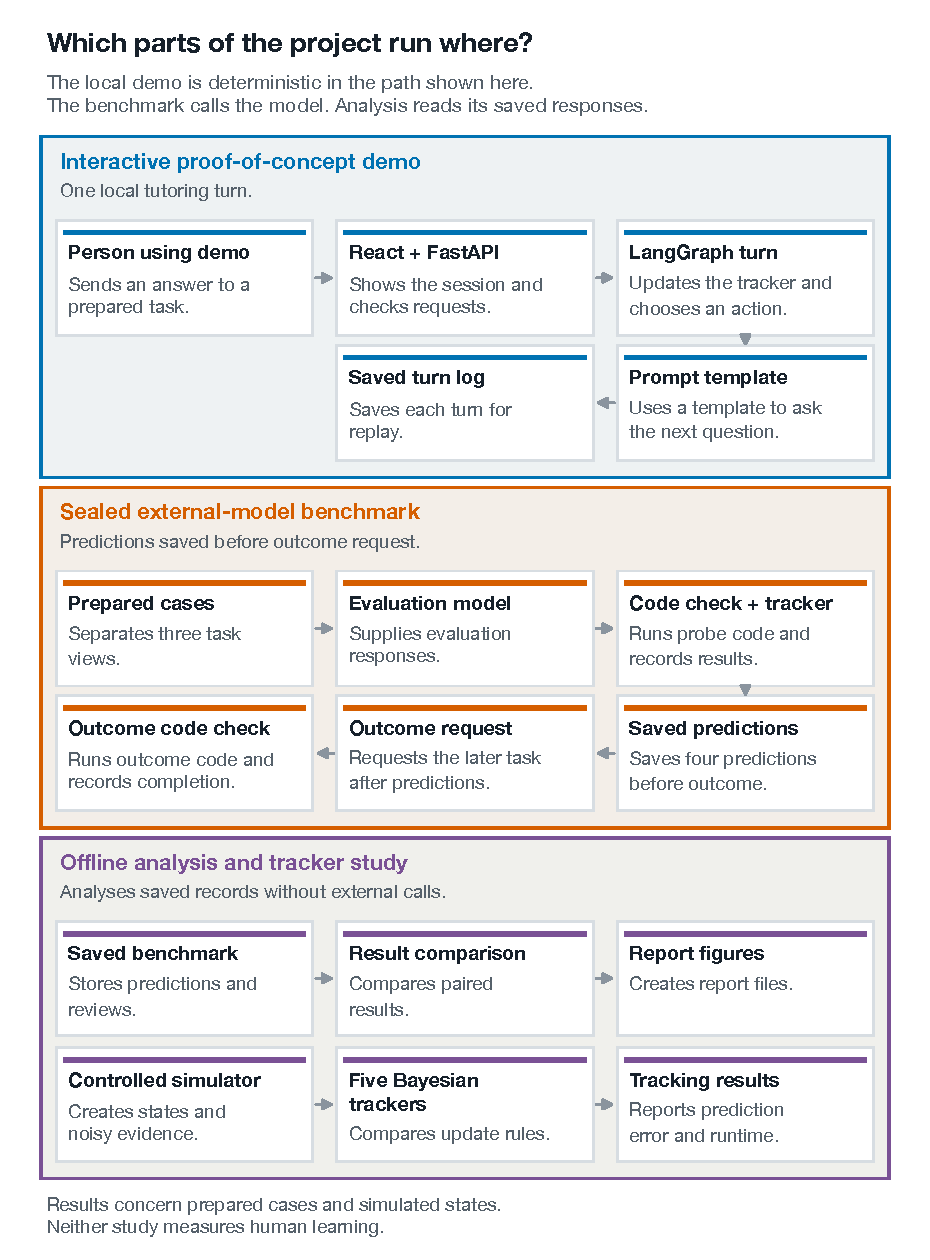
\includegraphics[width=\textwidth]{assets/figures/ch04-system/system_boundaries.pdf}
  \caption{The demonstration, external benchmark and Bayesian tracker study. The top row follows one local tutoring turn.
  The middle row shows the model and sandbox requests, with predictions saved before the outcome request. The bottom row
  shows analysis of saved records and simulated tracker updates. Probe selection and the CSEDM analysis are described separately
  in Chapter~\ref{ch:method}.}
  \label{fig:system-boundaries}
\end{figure}

\section{Engineering Choices}

Pixi fixes the Python and JavaScript environment. FastAPI and Pydantic provide typed API boundaries. React supplies the
examiner-facing interface. LangGraph makes the tutoring state transition explicit. Modal provides an external isolation boundary
for generated code. Saved local artefacts form the scientific record because they can be inspected and replayed without a
hosted dashboard.

\section{The Demonstration Turn}

The local graph makes one pass through evidence classification, tracker update, action selection, prompt generation and a
guardrail check. It has no retry cycle or autonomous planning loop. Each node returns its part of the state, and the final
contract rejects an incomplete result. A task and tracker with different concept identifiers are rejected before execution.

The classifier uses authored text markers. For configured follow-up questions, it uses the current tutor prompt to select
the applicable checks. On the initial question, a reply that matches an output marker but no explanation marker receives an
incomplete category.
The action policy then requests clarification. A recognised misconception receives a hint, while a recognised correct answer
leads to a transfer question. These categories describe matches to the configured rules. Unrecognised phrasing can leave a
valid answer unclassified, so the checker requires manual review of the intended demonstration paths.

The action policy receives the evidence category and observation number. It changes an uncertain observation to a
clarification action when the observation number exceeds three. The tracker score is displayed for inspection but does not
determine the action. Prompt generation uses the action, evidence category, current question and observation count to select
authored text. This provides a repeatable interaction for demonstrating the application. Its classification rules and score
changes have not been validated as measures of learner understanding.

\section{Prediction and Outcome Boundaries}

The benchmark gives the prediction process and evaluator different views of the case records. The prediction process receives
the visible evidence and initial tracker state. Its four conditions begin from the same state after the first answer. The
evaluator receives the later task outcome and uses it to score each prediction.

The system first checks that the input recordings contain no later task responses. It verifies the input hashes, executes
the evidence programs, saves the predictions and records missing cases. It then creates a global decision seal, a record

% TODO: clarify state transition constraints in LangGraph
